%! TEX root = **/010-main.tex
% vim: spell spelllang=ca :


\section{Resultats}%
\label{sec:resultats}

Tal com hem explicat als experiments, van acabar utilitzant una combinació de
diversos classificadors. Tot i que els resultats dels classificadors per separat
eren bastant satisfactoris, la combinació final no.

%Les matrius de confusió les mostrem en forma de gràfica. Les matrius completes
%es troben al \cref{sec:annex_matrius_conf}.

\subsection{Classificadors individuals}

\subsubsection{Classificador de senyals general}

\setcounter{MaxMatrixCols}{43}

Accuracy: 0.8836

\begin{equation*}
\begin{bmatrix}
2593	&	8	&	99	&	16	    &	5	&	7	&	8	&	5	&	3	&	0	&	16 \\
64	    &	157	&	2	&	16	    &	12	&	1	&	0	&	5	&	0	&	0	&	13 \\
222	    &	1	&	482	&	11	    &	2	&	0	&	0	&	1	&	0	&	0	&	1 \\
10	    &	0	&	9	&	1783	&	6	&	1	&	0	&	0	&	0	&	15	&	6 \\
30	    &	8	&	17	&	14	    &	337	&	9	&	1	&	0	&	4	&	0	&	0 \\
19	    &	2	&	5	&	14	    &	11	&	395	&	0	&	3	&	0	&	1	&	0 \\
10	    &	0	&	2	&	0	    &	2	&	0	&	154	&	0	&	12	&	0	&	0 \\
35	    &	1	&	14	&	0	    &	1	&	1	&	1	&	96	&	0	&	0	&	1 \\
1	    &	0	&	8	&	4	    &	7	&	2	&	6	&	0	&	212	&	0	&	0 \\
2	    &	0	&	0	&	87	    &	0	&	2	&	0	&	0	&	0	&	28	&	1 \\
48	    &	6	&	5	&	6	    &	3	&	0	&	0	&	0	&	0	&	0	&	1132
\end{bmatrix}
\end{equation*}

\subsubsection{Cercles Vermells i blancs}

Accuracy: 0.5855

\begin{equation*}
\begin{bmatrix}
    35	&	0	&	0	&	0	&	0	&	0	&	0	&	0	&	0	&	0	&	0 \\
4	&	308	&	27	&	16	&	11	&	53	&	5	&	9	&	0	&	0	&	0 \\
2	&	48	&	271	&	21	&	17	&	51	&	14	&	17	&	0	&	0	&	1 \\
4	&	15	&	16	&	138	&	11	&	30	&	9	&	10	&	0	&	0	&	4 \\
13	&	21	&	19	&	19	&	315	&	14	&	20	&	47	&	0	&	0	&	0 \\
1	&	27	&	58	&	57	&	24	&	194	&	25	&	30	&	0	&	0	&	0 \\
0	&	17	&	12	&	12	&	9	&	17	&	171	&	59	&	0	&	0	&	7 \\
1	&	11	&	23	&	17	&	20	&	13	&	37	&	109	&	0	&	0	&	0 \\
0	&	0	&	4	&	3	&	3	&	1	&	5	&	0	&	0	&	0	&	1 \\
0	&	3	&	20	&	16	&	10	&	17	&	13	&	18	&	0	&	0	&	2 \\
0	&	0	&	0	&	1	&	0	&	0	&	1	&	1	&	0	&	0	&	75 \\
\end{bmatrix}
\end{equation*}

\subsubsection{Cercles Blancs}

Accuracy: 0.6296

\begin{equation*}
\begin{bmatrix}
81	& 28	& 6	& 10 \\
4	& 23	& 12	& 20 \\
2	& 1	& 36	& 0 \\
3	& 8	& 6	& 30
\end{bmatrix}
\end{equation*}

\subsubsection{Cercles Blaus}

Accuracy: 0.9308

\begin{equation*}
\begin{bmatrix}
    149	&	0	&	0	&	0	&	0	&	1	&	1	&	0 \\
    149	&	0	&	0	&	0	&	0	&	1	&	1	&	0 \\
    0	&	67	&	1	&	0	&	1	&	2	&	0	&	4 \\
    1	&	7	&	238	&	0	&	0	&	11	&	0	&	4 \\
    0	&	4	&	0	&	89	&	0	&	5	&	0	&	0 \\
    0	&	1	&	0	&	0	&	58	&	0	&	0	&	1 \\
    0	&	11	&	1	&	1	&	1	&	377	&	0	&	1 \\
    0	&	0	&	0	&	0	&	0	&	0	&	59	&	0 \\
    0	&	0	&	0	&	0	&	0	&	24	&	0	&	80
\end{bmatrix}
\end{equation*}

\subsubsection{Triangles}

Accuracy: 0.7379

\begin{equation*}
\begin{bmatrix}
220	&	10	&	1	&	3	&	3	&	4	&	6	&	13	&	12	&	12	&	6	&	10	&	4	&	9	&	3 \\
6	&	210	&	0	&	5	&	1	&	11	&	0	&	8	&	7	&	17	&	2	&	9	&	1	&	0	&	14 \\
0	&	0	&	42	&	0	&	0	&	1	&	1	&	0	&	0	&	0	&	0	&	0	&	0	&	0	&	0 \\
1	&	2	&	0	&	48	&	0	&	3	&	1	&	1	&	0	&	0	&	2	&	2	&	3	&	0	&	0 \\
1	&	1	&	7	&	1	&	72	&	1	&	0	&	1	&	0	&	1	&	0	&	0	&	0	&	0	&	1 \\
2	&	1	&	0	&	1	&	0	&	29	&	0	&	0	&	0	&	0	&	0	&	0	&	1	&	2	&	0 \\
4	&	1	&	5	&	9	&	1	&	12	&	78	&	0	&	1	&	0	&	0	&	0	&	1	&	0	&	5 \\
0	&	2	&	0	&	0	&	1	&	0	&	0	&	19	&	0	&	0	&	0	&	0	&	0	&	0	&	0 \\
16	&	6	&	0	&	16	&	0	&	9	&	3	&	2	&	263	&	2	&	3	&	3	&	2	&	5	&	8 \\
9	&	3	&	0	&	3	&	2	&	3	&	4	&	0	&	2	&	78	&	5	&	0	&	4	&	1	&	1 \\
2	&	0	&	0	&	0	&	0	&	0	&	0	&	2	&	0	&	4	&	38	&	0	&	0	&	0	&	1 \\
3	&	2	&	0	&	2	&	0	&	0	&	6	&	2	&	4	&	1	&	1	&	93	&	3	&	0	&	0 \\
0	&	0	&	0	&	0	&	0	&	0	&	8	&	0	&	1	&	0	&	0	&	1	&	34	&	0	&	1 \\
5	&	2	&	1	&	2	&	4	&	15	&	9	&	10	&	9	&	3	& 0	&	2	&	0	&	73	&	4 \\
1	&	0	&	4	&	0	&	6	&	2	&	4	&	2	&	1	&	2	& 3	&	0	&	7	&	0	&	142 \\
\end{bmatrix}
\end{equation*}

\subsection{Classificadors combinats}

Accuracy: 0.5529

\begin{figure}[H]
\centering
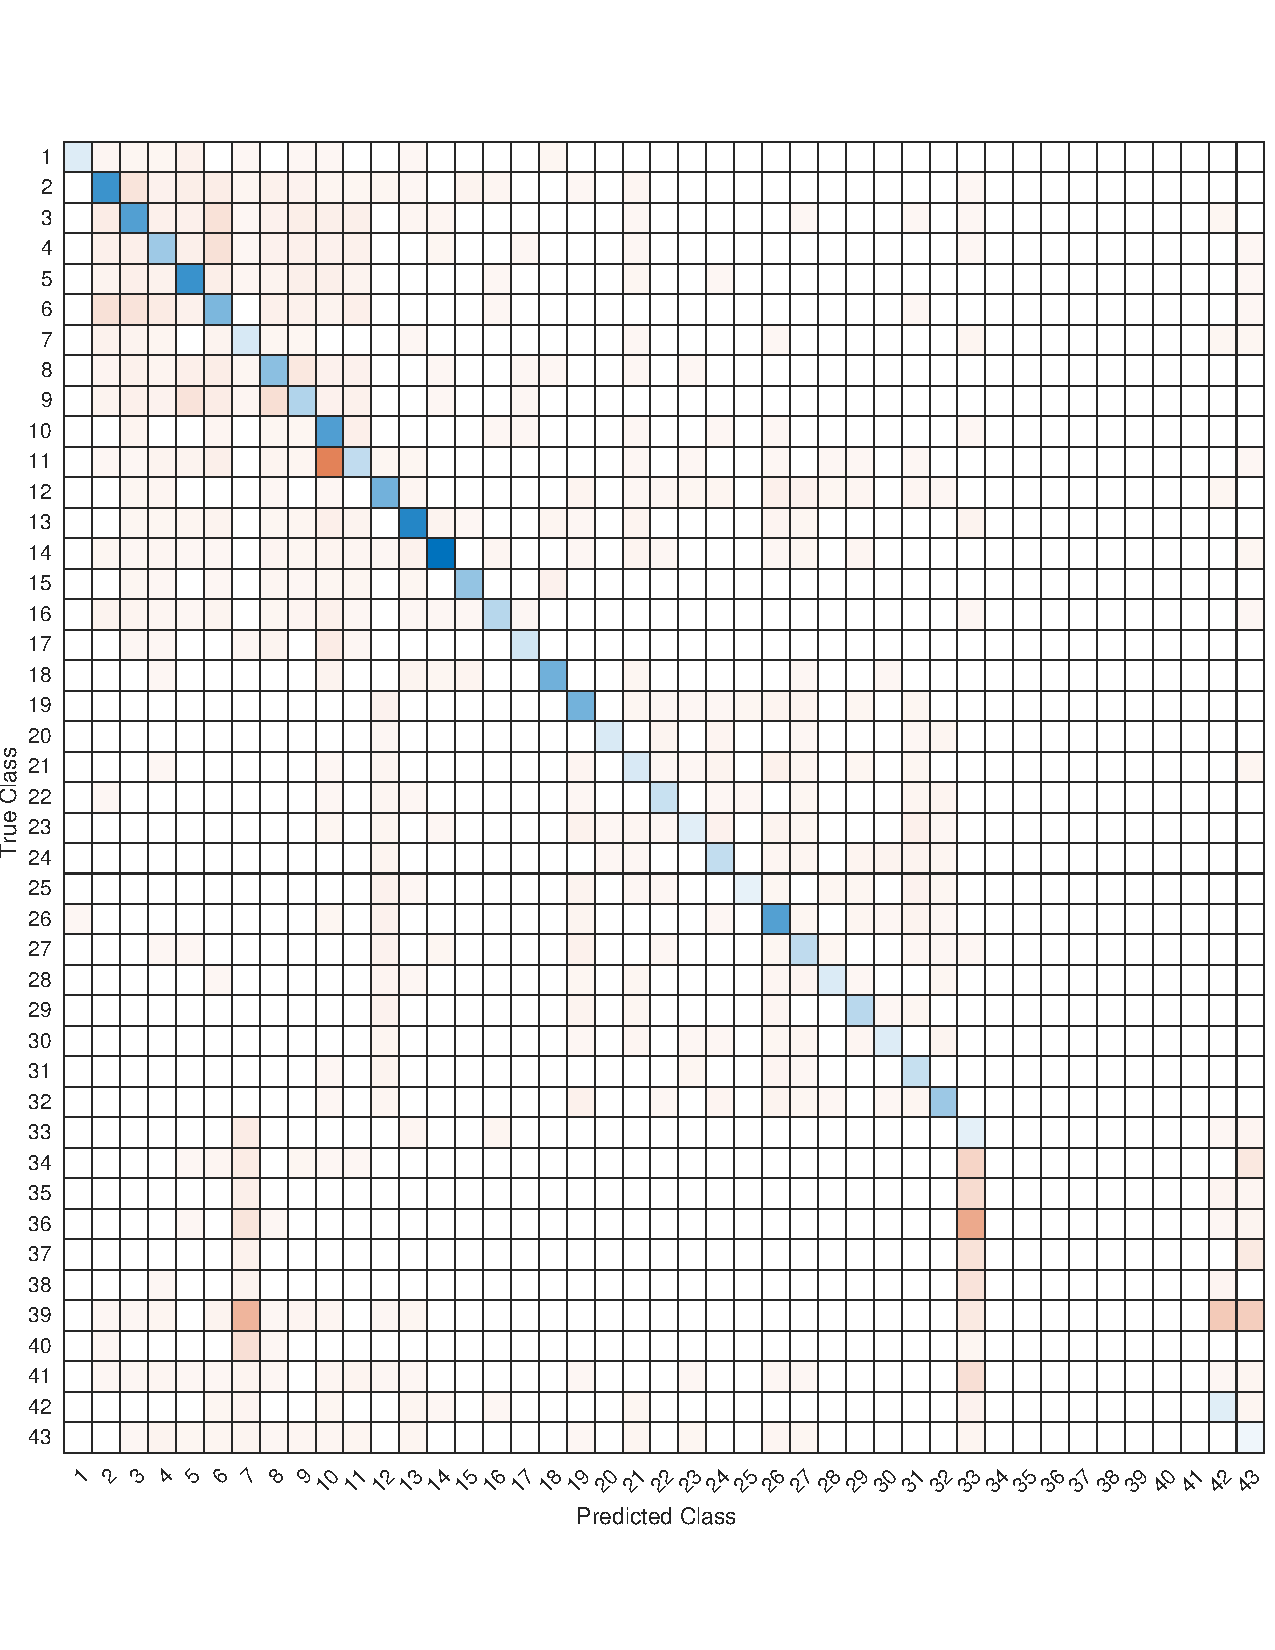
\includegraphics[width=0.9\textwidth]{confusion_chart_general}
\caption{Gràfica de la matriu de confusió}%
\label{fig:conf_chart}
\end{figure}

La matriu sencera es troba al \cref{sec:ann:mat}.
